\documentclass{itatnew}
\usepackage{todonotes}
\usepackage{soul}
\presetkeys{todonotes}{inline}{}
\presetkeys{todonotes}{prepend}{}
\presetkeys{todonotes}{caption=TODO}{}
\def\VH#1{\textcolor{cyan}{VH: \textit{#1}}}
\def\OP#1{\textcolor{purple}{OP: \textit{#1}}}
% \def\OP#1{\relax}  % make my comments vanish completely
\def\PB#1{\textcolor{red}{PB: \textit{#1}}}
\def\todo#1{\textcolor{purple}{todo: \textit{#1}}}

\definecolor{darkgreen}{rgb}{0.0, 0.5, 0.0}
\def\OD#1{{\color{darkgreen}OD: \it #1}}
\usepackage[normalem]{ulem}
\def\ODdel#1{\bgroup\markoverwith{\textcolor{darkgreen}{\rule[0.5ex]{2pt}{1pt}}}\ULon{#1}}
%\def\OD#1{\relax} % make my comments vanish
%\def\ODdel#1{#1} % make my comments vanish


\def\area#1{{\color{darkgreen}area:\it #1}}
\def\food#1#2{{Dial. state #1: \color{blue}food:\it #2}}
\def\pricerange#1{{\color{orange}pricerange:\it #1}}
\def\sys#1{{\color{purple}System: \it #1}}
\def\usr#1{{\color{brown}User: \it #1}}

\begin{document}

\title{Recurrent Neural Networks for Dialogue State Tracking}

\author{Ondřej Plátek \and Petr Bělohlávek \and Vojtěch Hudeček  \and Filip Jurčíček}

\institute{Charles University in Prague, Faculty of Mathematics and Physics \\
\email{\{oplatek,jurcicek\}@ufal.mff.cuni.cz},\\
\email{me@petrbel.cz},\\
\email{vojta.hudecek@gmail.com},\\
\texttt{http://ufal.mff.cuni.cz/ondrej-platek}}

\maketitle              % typeset the title of the contribution

%% REVIEWERS comments %%%%%%%%
% \OP{not standard metric and comparison to other systems \\} - DONE
% \OP{reference na dstc2 - todo provide link to footnote \\} - DONE
% \OP{Predstavit DST co to je - summarizing dialogue history in formal state} - DONE? - have no space/skills to do it better \\
% \OP{Opravit vetu "A dialogue state tracker summarizes the hidden information state (HIS)\cite{young2010hidden} of a user's goal from the conversation history." - reviewer alergicky na ni} - DONE\\
% \OP{jak pouzivane rnn} - DONE \\
% \OP{sekce 3 zacina bez uvodu do modelu} - Not sure what can I do with it - no space \\
% \OP{vysvetlit zkratky ASR a GRU} - DONE \\
% \OP{kde jsem vzal database} - DONE \\
% \OP{whe seq2seq generates 3 labels + EOS} - DONE \\
% \OP{why not ASR n-best list} - DONE \\
% \OP{example dialogue state task} - DONE
% \OP{why not slots name - name is in the dataset but not used for evaluation - only slots which are informable} - DONE \\
% \OP{no incremental - true but no validation set} - DONE \\
%% End of REVIEWERS comments %%%%%%%%

%%%% MY TODO %%%%
% \OP{jak dlouho trvala epocha - proc je tak pomala? \\}
% \OP{accuracies on train set \\}  - not time
% \OP{myslim, ze to mam dobre, ale v camera ready to zkontrolujem - nestiham. \PB{nemusi byt podekovani metacentru v nejake jejich oficialni podobe - link v komentari?} \url{https://wiki.metacentrum.cz/wiki/Pravidla-BLABLA}} - Done
%%% END OF MY TODO %%%


\begin{abstract}
This paper discusses models for dialogue state tracking using recurrent neural networks (RNN).
We present experiments on the standard dialogue state tracking (DST) dataset, DSTC2~\cite{henderson2014second}.
On the one hand, RNN models became state of the art in DST,
on the other hand, most state-of-the-art models are only turn-based and require dataset-specific preprocessing (e.g. DSTC2-specific) in order to achieve state-of-the-art results.
We implemented two architectures which can be used in incremental settings and require almost no preprocessing.
We compare their performance to the benchmarks on DSTC2 and discuss their properties.
With only trivial preprocessing, the performance of our models is close to the state-of-the-art results.\footnote{
    {\bf Acknowledgment:} We thank Mirek Vodolán and Ondřej Dušek for useful comments.
    This research was partly funded by the Ministry of Education, Youth and Sports of the Czech Republic under the grant agreement LK11221, core research funding, grant GAUK 1915/2015, and also partially supported by SVV project number 260 333. 
    We gratefully acknowledge the support of NVIDIA Corporation with the donation of the Tesla K40c GPU used for this research.
    Computational resources were provided by the CESNET LM2015042 and the CERIT Scientific Cloud LM2015085, provided under the programme ``Projects of Large Research, Development, and Innovations Infrastructures''.
    }
\end{abstract}

\section{Introduction}
 
This paper compares two different RNN architectures for dialogue state tracking (see Section~\ref{sec:model}).
We describe state-of-the art word-by-word dialogue state trackers architectures and propose to use a new encoder-decoder architecture for the DST task (see Section~\ref{sec:eval}).
First, we briefly introduce dialogue state tracking.

Dialogue state tracking (DST) is a standard and important task for evaluating task-oriented conversational agents~\cite{williams2013dialog, henderson2014second, henderson2014third}.
Such agents play role of domain expert on narrow domain and users ask for information through conversation in natural language (see system and user responses in~Figure~\ref{fig:example}).
A dialogue state tracker summarizes the dialogue history and maintains distribution over user's goal (see annotation in~Figure~\ref{fig:example}).
Dialogue agents as introduced in~\cite{young2010hidden} decide about next action based on the dialogue state distribution from the tracker.
User's goals are expressed in a~formal language, typically represented as a dialogue act item (DAI) and the tracker updates probability for each item. 
Since the dialogue state is a latent variable it is called a~hidden information state (HIS)~\cite{young2010hidden} and one needs to label conversation to train a dialogue state tracker using supervised learning.
It was shown that with a better dialogue state tracker, conversation agents achieve better success rate in overall completion of the their task~\cite{jurvcivcek2012reinforcement}.

\begin{figure}
   \dots \\
    \food{n}{None}, \area{None}, \pricerange{None} \\
    \sys{What part of town do you have in mind?} \\
    \usr{West part of town.} \\
    \food{n+1}{None}, \area{west}, \pricerange{None} \\
    \sys{What kind of food would you like?} \\
    \usr{Indian} \\
    \food{n+2}{Indian}, \area{west}, \pricerange{None} \\
    \sys{India House is a nice place in the west of town serving tasty Indian food.} \\
    \dots
    \caption{Example of golden annotation of Dialogue Act Item (DAI). The dialogue act item comprises from act type (all examples have type {\it inform}) and slots ({\it food, area, pricerange}) and their values (e.g. {\it Indian, west, None}).}
\vspace{-0.70em}
\label{fig:example}
\end{figure}

We focus only on the {\it goal} slot predictions because the other groups are trivial to predict\footnote{The slots {\it Requested} and {\it Method} have accuracies 0.95 and 0.95 on the test set according to the state-of-the-art~\cite{williams2014web}.}.

We also experiment with re-splitting of the DSTC2 data because there are considerable differences between the standard train and test data sets~\cite{henderson2014second}.
Since training, development and test set data is distributed differently, the resulting performance difference between training and test data is rather high.
Based on our experiments, we conclude that DSTC2 might suggest too pessimistic view of the state-of-the-art methods in dialogue state tracking caused by the data distribution mismatch.


\section{Dialogue state tracking on DSTC2 dataset}\label{sec:dst}
Dialogue state trackers maintain their believes about users goals by updating probabilities of dialogue history representations.
In the DSTC2 dataset, the history is captured by dialogue act items and their probabilities.
A Dialogue act item is a triple of the following form $(actionType, slotName, slotValue)$.

The DSTC2 is a standard dataset for DST, and most of state-of-the-art systems in DST have reported their performance on~this dataset~\cite{henderson2014second}. 
The full dataset is freely available since January 2014 and contains 1612 dialogues in the training set, 506 dialogues in the development set and 1117 dialogues in the test set.\footnote{Available online at~\url{http://camdial.org/~mh521/dstc/}.}
The conversations are manually annotated at the turn level where the hidden information state is expressed in form of $(actionType, slotName, slotValue)$ based on the~domain ontology.
The task of the domain is defined by a~database of restaurants and their properties\footnote{There are six columns in the database: name, food, price\_range, area, telephone, address.}.
The~database and a~manually designed ontology which captures a~restaurant domain are distributed with the dataset.

\section{Models}\label{sec:model}
Our models are all based on a RNN encoder~\cite{werbos1990backpropagation}. 
Similarly to RNN encoder of~\cite{zilka2015incremental}, the models update their hidden states $h$ after processing each word. 
The encoder takes as inputs the previous state $h_{t-1}$ representing history for first $t-1$ words and features $X_t$ for the current word $w_t$. 
It outputs state $h_t$ representing the whole dialogue history up to current word.
We use a~Gated Recurrent Unit (GRU) cell~\cite{cho2014gru} as the update function instead of simple RNN cell because it does not suffer from vanishing gradient~\cite{TODO_vanishing_gradient}.
The model optimizes its parameters during training.

For each input token, our RNN encoder reads the word embedding~\cite{bengio2003neural} of this token along with several binary features. 
The binary features for each word are:
\begin{itemize}
	\item the speaker role, representing either user or system,
    \item and also indicators describing whether the word is part of some named entity representing a value from the database.
\end{itemize}
Since DSTC2 database is a simple table with six columns, we introduce six binary features firing if the word is a substring of named entity at given column.
For example, the word {\it indian} will not only trigger the feature for column $food$ and its value {\it indian} but also for column restaurant $name$ and its value {\it indian heaven}.
The features make the data dense by abstracting the meaning from lexical level. 

Our model variants differ only in the way they predict {\it goal} labels, i.e. $food$, $area$ and $price range$ from the RNN's last encoded state.\footnote{Accuracy measure with schedule 2 on slot $food$, $area$ and $price range$ about which users can inform the system is a featured metric for DSTC2 challenge~\cite{henderson2014second}.} 
% The first model predicts the triples of slot values $(food, area, price range)$ jointly from the encoder hidden state $h$.
The first model predicts the output slot labels independently by employing three independent classifiers (see Section~\ref{sec:indep})
The second model uses a decoder in order to predict values one after each other from the $h_{T}$ (see Section~\ref{sec:encdec}).
% We also experimented with single classifier which predicts the labels jointly (see Figure~\ref{fig_encjoint}, but it suffers from data sparsity of the predicted tuples, so we focused only on the independent label prediction and encoder-decoder models.
We also experimented with single classifier which predicts the labels jointly (see Figure~1, but it suffers from data sparsity of the predicted tuples, so we focused only on the independent label prediction and encoder-decoder models.

The models were implemented using TensorFlow~\cite{abaditensorflow} framework. 
By introducing encoder-decoder architecture, we aim to overcome the data sparsity problem and incorrect independence assumptions.

\begin{figure}
\vspace{-0.80em}
\begin{center}
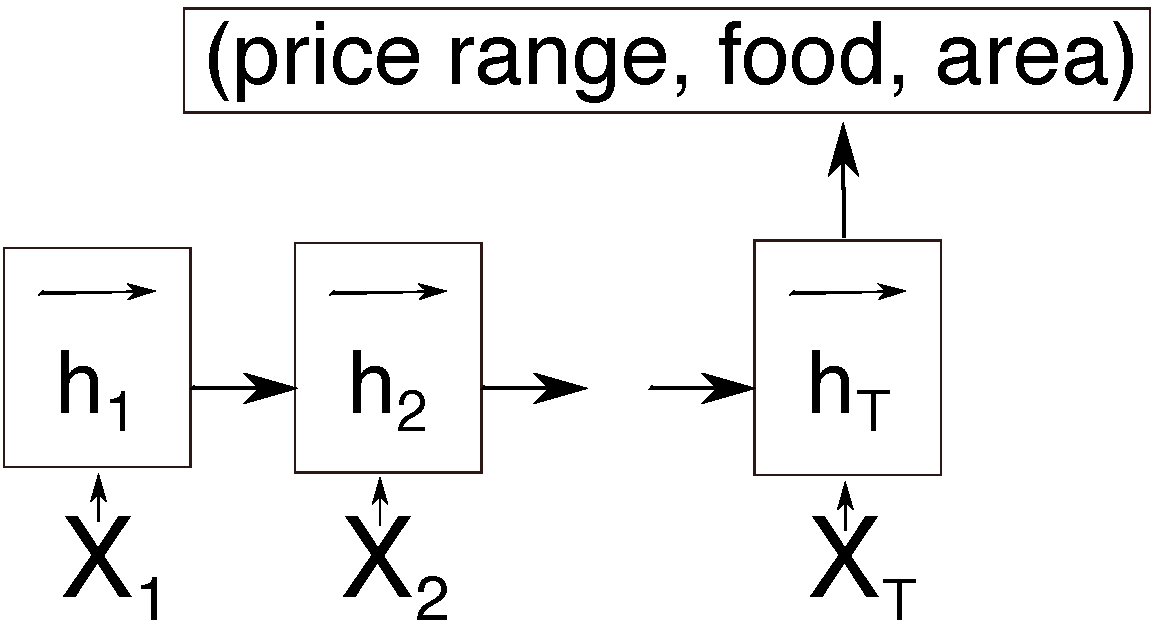
\includegraphics[height=9em]{encoder_joint}
\caption{The joint label predictions using RNN from last hidden state $h_T$. The $h_T$ represents the whole dialog history of $T$ words. The RNN takes as input for each word $i$ an embedding and binary features concatenated to~vector~$X_{i}$.}
\end{center}
\vspace{-0.70em}
\label{fig_encjoint}
\end{figure}

\subsection{Independent classifiers for each label}
\label{sec:indep}
The independent model predicts slots $food$, $area$ and $price range$ based on the last hidden state $h_{T}$ independently using three classifiers.
Independent slots prediction using one classifier per each slot is straightforward to implement, but the model introduces an unrealistic assumption of uncorrelated slot properties.
In case of DSTC2 and the Cambridge restaurant domain, it is hard to believe that, e.g., the slots $area$ and $price range$ are not correlated.

\begin{figure}
\begin{center}
\includegraphics[height=9.5em]{encoder}
\caption{The RNN encodes the word history into dialogue state $h_T$ and predicts slot values independently.}
\end{center}
\vspace{-0.80em}
\label{fig:encind}
\end{figure}

\subsection{Encoder-decoder framework}
\label{sec:encdec}
The encoder-decoder model with attention~\cite{bahdanau2014neural} is the most sophisticated model that we used for slot predictions.
To our knowledge, we are first who used this model for the task of slot predictions.
The model is successfully used in machine translation where it is able to handle long sequences with good accuracy.
In DST, it captures correlation between the decoded slots easily~\cite{bahdanau2014neural}. 

We use the encoder RNN cell captures the history of a dialogue which is represented as a~sequence of words from user and system.
The words are fed to the encoder as they appear in dialogue turn by turn where user and system responses switch regularly.
The encoder updates its internal state $h_T$ after each word.
The RNN decoder model is used when the system needs to generate its output, in our case it is at the end of the user response.
The decoder generates arbitrary length sequence of words takes given the encoded state $h_T$ step by step.
In each step, an output word and a~new hidden state $h_{T+1}$ is generated.
The generation process is finished when a special token End of Sequence (EOS) is generated.
The attention part of model is used at decoding time for weighting the importance of the history. 

The disadvantage of this model is its complexity.
Firstly, the model is not trivial to implement\footnote{We modified code from the TensorFlow `seq2seq` module.}. 
Secondly, the decoding time is quadratic in the length of the decoded sequences, but our target sequences are only four tokens long.
%\PB{In contrast, the decoding consumes asymptotically constant time regardless the input.}  to mi prijde zbytecny, to ocekavas.
\begin{figure}
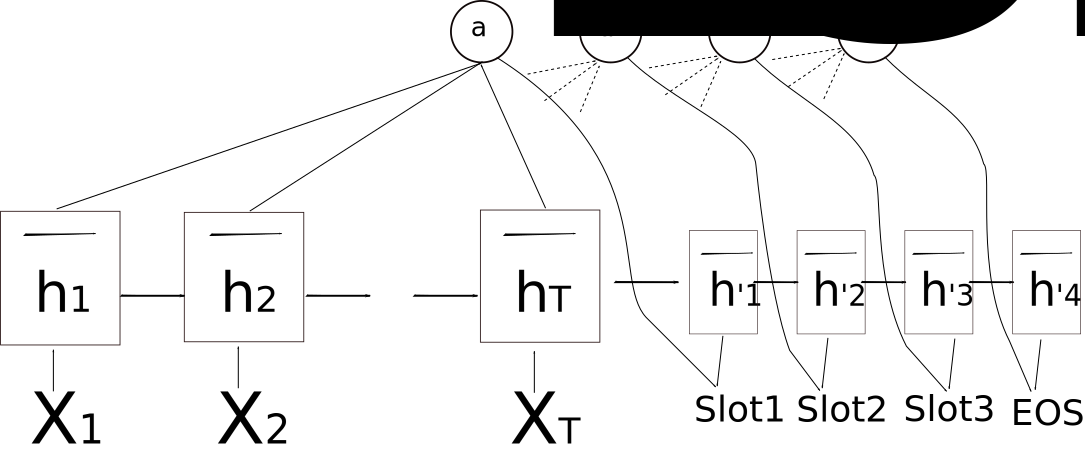
\includegraphics[width=0.5\textwidth]{encdec}
\caption{Encoder decoder with attention predicts goals.}
\label{fig:encdec}
\end{figure}

\section{Experiments}\label{sec:exp}
We report results on the standard DSTC2 data split where we used 516 dialogues as a validation set for early stopping~\cite{prechelt1998early} and the remaining 1612 dialogues for training.
We use 1-best Automatic Speech Recognition (ASR) transcriptions of conversation history on the input and measure joint slot accuracy.
We evaluate the models using the recommended measure accuracy with schedule 2 which skips the first turns where the believe tracker does not track any values. 
In addition, the models are evaluated on a randomly split DSTC2 dataset (see Section~\ref{sec:split}).

For all our experiments, we train word embeddings of size 100 and use the encoder state size of size 100, together with a dropout keep probability of $0.7$ for both encoder inputs and outputs.
These parameters are selected by a grid search over the hyper-parameters on development data.

\subsection{Training}
\label{sec:train}
The training procedure minimizes the cross-entropy loss function using the Adam optimizer~\cite{kingma2014adam} with a batch size of 10.
We train predicting goal slot values for each turn.
We treat each dialogue turn as a separate training example, feeding the whole dialogue history up to the current turn into the encoder and predicting the slot labels for the current turn.

We use early stopping with patience~\cite{prechelt1998early}, validating on the development set after each epoch and stopping if the three top models does not change for four epochs.

The predicted labels in DST task depend not only on the last turn, but on the dialogue full history as well.
Since the lengths of dialogue histories vary a lot\footnote{The maximum dialogue history length is 487 words and 95\% percentile is 205 words for the training set.} and we batch our inputs, we separated the dialogues into ten buckets accordingly to their lengths in order to provide a computational speed-up. We reshuffle the data after each epoch only within each bucket.

In informal experiments, we tried to speed-up the training by  optimizing the parameters only on the last turn\footnote{The prediction was conditioned on the full history but we back-propagated the error only in words within the last turn.} but the performance dropped relatively by more than 40\%.

\subsection{Comparing models}
\label{sec:eval}

Predicting the labels jointly is quite challenging because the distribution of the labels is skewed as demonstrated in~Figure~\ref{fig:labels}.
Some of the labels combinations are very rare, and they occur only in the development and test set so the joint model is not able to predict them.
During first informal experiments the~joint model performed poorly arguably due to data sparsity of slot triples. We further focus on model with independent classifiers and encoder-decoder architecture.

\begin{figure}
\vspace{-0.80em}
    \begin{center}
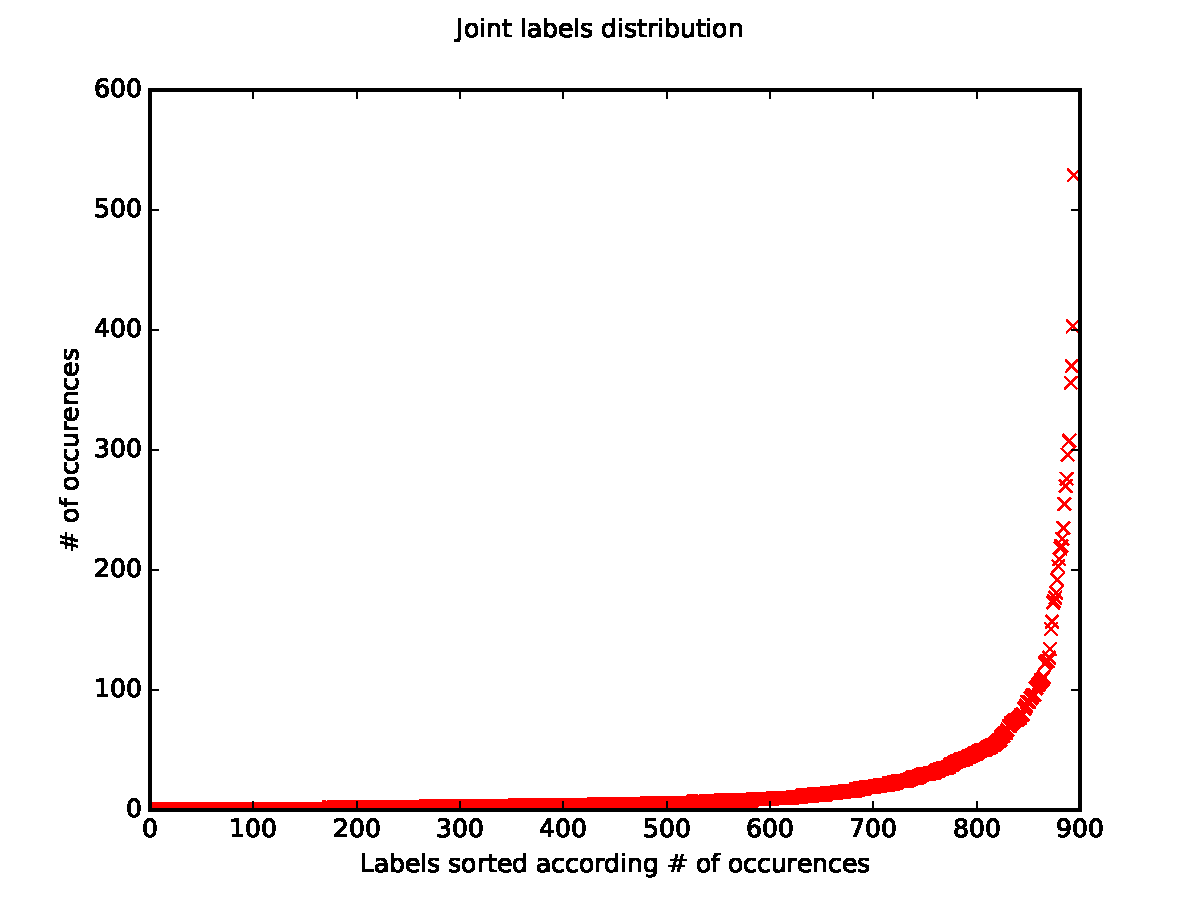
\includegraphics[width=0.4\textwidth]{jointLabelsDistrib}
    \end{center}
\vspace{-1.80em}
\caption{The number occurrences of labels in form of $(food, area, pricerange)$ triples from the least to the most frequent.}
\label{fig:labels}
\end{figure}

% The model with independent label prediction obtained much better performance on each slot individually as expected, but also it surprisingly outperformed the joint model in the joint prediction.
% We hypothesize that with larger amount of data the joint model would suffer less from data sparsity and perform better.
% This claim is supported by comparison of joint and independent models performance on the original DSTC2 dataset.
The model with independent label prediction is a strong baseline which was used, among others, in work of~\cite{zilka2015incremental}.
The model suffers less from data set mismatch because it does not model the correlation between predicted labels.
This property can explain a smaller performance drop between the test set from reshuffled data and the official test set in comparison to encoder-decoder model.

% FIXME include results from other papers
\begin{table}
\vspace{-0.80em}
\begin{center}
\begin{tabular}{l@{\quad}rll}
\hline
\multicolumn{1}{l}{\rule{0pt}{12pt}
                   Model}&\multicolumn{1}{l}{Dev set}&\multicolumn{2}{l}{Test set}\\[2pt]
\hline\rule{0pt}{12pt}
% Joint  &  todo &  todo \\
% /a/SSD/oplatek/e2end/log/2016-06-08-17-31-38.400-dstc-INDEP_labels-d0.7-w100-e100/
% /a/SSD/oplatek/e2end/log/TEST-ORIGINAL-2016-06-08-17-31-38.400dstc-INDEP_labels-d0.7-w100-e100-reward-0.9080-step-0036224
    Indep  &   \OP{0.91} & 0.727 \\
    EncDec &   \OP{0.94} & \OP{0.73} \\
\hline
    Vodolán et al.~\cite{vodolan2015hybrid} & - & 0.745 \\
    Žilka, Jurčíček~\cite{zilka2015incremental} & 0.69 & 0.72 \\
    Henderson et al.~\cite{henderson2013deep} & - & 0.737 \\
\hline
    DSTC2 stacking ensemble~\cite{henderson2014second} & - & 0.789 \\
\hline
\end{tabular}
\caption{Accuracy on DSTC2 dataset. The first group contains our systems which use ASR output as input, the second group lists systems using also ASR hypothesis as input. The third group shows the results for ensemble model using ASR output nd also live language understanding annotations.}
\vspace{-2em}
\end{center}
\label{tab:dstc}
\end{table}

Since the encoder-decoder architecture is very general and can predict arbitrary output sequences, it also needs to learn how to predict only three slot labels in the correct order.
It turned out that the architecture learned to predict quadruples with three slot values and the EOS symbol quickly, even before seeing a~half of the training data in the first epoch.\footnote{We could have modified the decoder to always predict three symbols for our three slots, but our experiments showed that the encoder-decoder architecture does not make mistakes at predicting the order of the three slots and EOS symbol.}  
At the end of the first epoch, the system made no more mistakes on predicting slot values in the incorrect order.
The encoder-decoder system is competitive with state-of-the art architectures and the time needed for learning the output structure was surprisingly short.\footnote{The best model weights were found after 18 to 23 epochs for all model architectures.}
% \OP{significance testing and fine tuning enc-dec vs others}

\subsection{Data preparation experiments}
\label{sec:split}

% FIXME include results from other papers
\begin{table}
\vspace{-0.20em}
\begin{center}
\begin{tabular}{l@{\quad}rll}
\hline
\multicolumn{1}{l}{\rule{0pt}{12pt}
                   Model}&\multicolumn{1}{l}{Dev set}&\multicolumn{2}{l}{Test set}\\[2pt]
\hline\rule{0pt}{12pt}
% Joint  &  todo &  todo \\
Indep  &   0.87 & 0.89 \\
EncDec &   0.94 & 0.91 \\
\hline
\end{tabular}
\caption{Accuracy of our models on the re-split DSTC2 data.}
\vspace{-2em}
\end{center}
\label{tabsplit}
\end{table}

The data for the DSTC2 test set were collected using a different spoken dialogue system configuration than the data for the validation and the training set.\cite{henderson2014second}.
We wanted to investigate how this influences the complexity of the task so we merged all DSTC2 data together and created splits of 80\%, 10\% and 10\% for the training, development and test sets.
% The~results in Table~\ref{tabsplit} show that the complexity of the task dropped significantly.
The~results in Table~2 show that the complexity of the task dropped significantly.


\section{Related work}\label{sec:related}
There are numerous systems which reported on the DSTC2 dataset, we discuss only the systems which use RNNs.
In general, the RNN systems achieved excellent results.

Our system is related to the RNN tracker of Žilka and Jurčíček~\cite{zilka2015incremental},
which reported near state-of-the art results on the~DSTC2 dataset and was the first incremental system which was able to update the dialogue state word-by-word with such accuracy.
In contrast to work of~\cite{zilka2015incremental}, we use no abstraction of slot values. 
Instead, we add the additional features as described in Section~\ref{sec:model}.
The first system which used a neural network for dialogue state tracking~\cite{henderson2013deep} used a feed-forward network and more than 10 manually engineered features across different levels of abstraction of the user input, including outputs of the spoken language understanding component (SLU).
In our work, we focus on simplifying the architecture, hence we used only features which were explicitly given by the dialogue history word representation and the database.

The system of Henderson et al.~\cite{henderson2014word} achieves state-of-the-art results and, similarly to our system, it predicts the dialogue state from words by employing a RNN.
On the other hand, their system heavily relies on the user input abstraction.
Another dialogue state tracker with LSTM was used in reinforcement setting but the authors also used information from the SLU pipeline~\cite{lee2016dialog}.

An interesting approach is presented in the work of Vodolán et al.~\cite{vodolan2015hybrid}, who combine a rule-based and a machine learning based approach.
The handcrafted features are fed to an LSTM-based RNN which performs a dialog-state update.
However, unlike our work, their system requires SLU parses on the input.

It is worth noting that there are first attempts to train an end-to-end dialogue system even without explicitly modeling the dialogue state~\cite{bordes2016learning}, which further simplifies the architecture of a dialogue system.
However, the reported end-to-end model was evaluated only on artificial dataset and cannot be compared to DSTC2 dataset directly.

\section{Conclusion}\label{sec:conc}
We presented and compared two dialogue state tracking models which are based on state-of-the-art architectures using recurrent neural networks.
To our knowledge, we are the first to use an encoder-decoder model for the dialogue state tracking task, and we encourage others to do so because it is competitive with the standard RNN model.\footnote{The presented experiments are published at \url{https://github.com/oplatek/e2end/} under Apache license. Informal experiments were conducted during the Statistical Dialogue Systems course at Charles University (see \url{https://github.com/oplatek/sds-tracker}).}
The models are comparable to state-of-the-art.

We evaluated the models on DSTC2 dataset containing task-oriented dialogues in restaurant domain. 
We trained the models using only ASR 1-best transcriptions and task-specific lexical features defined by the task database.
We observed that dialogue state tracking on DSTC2 test set is notoriously hard and that the task becomes substantially easier if the data is reshuffled.

As future work, we plan to investigate influence of the introduced database features on models accuracy.
To our knowledge there is no dataset which can be used for evaluating incremental dialogue state trackers, so it would be beneficial to collect annotation on word level so one can evaluate incremental DST models.

\newpage
\bibliographystyle{plain}
\bibliography{samplearticle}
\end{document}
